\chapter{Patient}
Ved implementering af en ny teknologi, herunder en Ultralyds Robotarm, kan det have en indvirkning på patienten. Derfor er det vigtig at belyse, hvilken effekt den nye teknologi har på patientgruppen. \\
I denne MTV vil både gravide og sonografer blive placeret i rollen som patienter. Gravide da de får foretaget en ultralydscanning og sonografer da de ofte oplever arbejdskader. Begge grupper vil derfor blive belyst i dette afsnit.  \\ \newline
Dette afsnit vil delvist være baseret på et interview og efterfølgende samtaler med sonografer på Horsens Sygehus og Viborg Regionshospital. 
\newline
For at kunne udarbejde en fyldestgørende analyse af patientperspektivet er det nødvendigt at belyse flere forhold. Se figur \ref{patientMTV}, hvor de fem patientperspektiver er vist. 
\begin{figure}[h!]\centering
	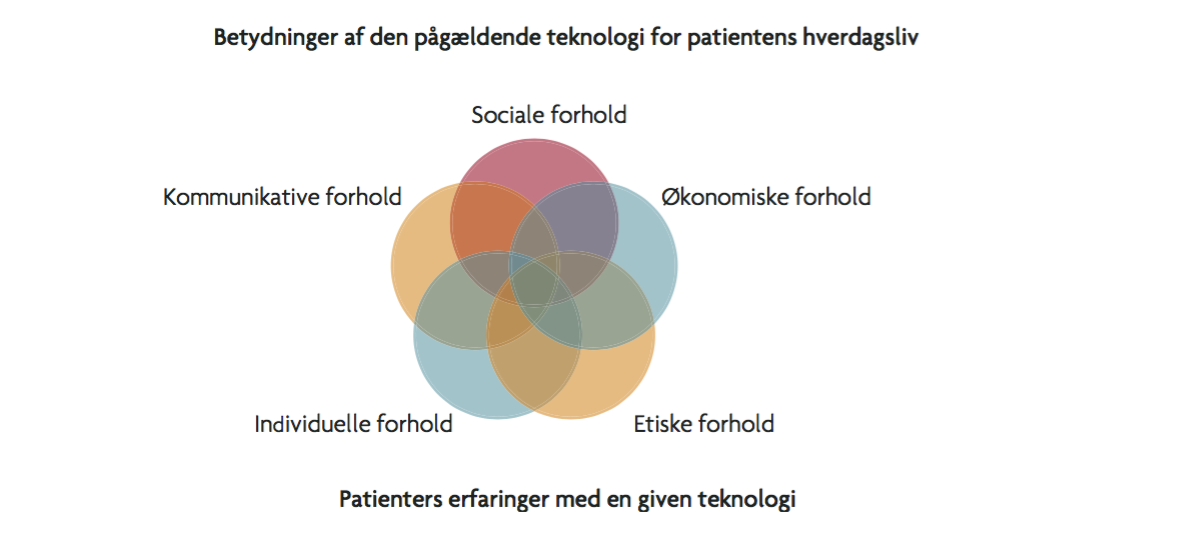
\includegraphics[width = 1.0\textwidth]{Figurer/PatientaspekterMTV}
	\caption{Udforskning af de fem patientaspekter i MTV, som har betydning for patientens hverdagsliv}
	\label{patientMTV}
\end{figure}

\section{Sociale forhold}
På nuværende tidspunkt findes skepsis blandt sonografer i forhold til om de kan forsætte med at scanne indtil pensionsalderen. Godt 20 \% kommer på førtidspension grundet deres arbejde ifølge \cite{BeckyMorton2007}. \\ 
For personalet vil eventuelle færre arbejdsskader betyde et større udbytte af fysiske funktioner i forhold til arbejde, men også i fritiden. Dette kan forlænge tiden på arbejdsmarkedet og forbedre personalemiljøet.       

\section{Kommunikative forhold}
Produktet af scanningen, eksempelvis billeder og kønsbestemmelse, vil ikke blive påvirket af Ultralyds Robotarmen.
For personalet vil det kræve en anden introduktion, da de ikke længere vil have den fysiske kontakt med den gravide. Derved er den gravide selv nødsaget til at meddele ubehag.  \\
Personalet vil igennem bedre arbejdsstillinger muligvis opleve et andet overskud til arbejdssituationen og patientkontakten.  

\section{Individuelle forhold}
Den gravide patient kan måske opleve en utryghed ved at få en fremmed teknologi, Robotarmen, fysisk tæt på sig. Dette kan forøge den utryghed som den gravide i forvejen kan have i første trimester omkring sikkerheden af en ultralydsscanning \cite{Lea1985}.Der vil altid være personale tilstede under en scanning, som skaber en menneskelig kontakt og en professionel tryghed.  \\
Personalets anciennitet vil være en stor tryghedsfaktor for patienten. Derved vil en eventuel utryghed fra den gravide patient blive mindsket når personalet udviser sikkerhed og åbenhed for teknologien.\\
For den gravide er det især vigtigt at knytte bånd med fosteret. Derved mente sonograferne på Viborg, at så længe de gravide kunne se fosteret på skærmen, ville den nye teknologi ikke have stor påvirkning. \\  
Personalet er meget engagerede i deres arbejde, hvilket kan være en af grundene til at de ikke indmelder skader. Dette er på trods af undersøgelser som viser at mange sonografer døjer med smerter \cite{BeckyMorton2007}. 
Hvis akavet og fysisk udfordrende arbejdsstillinger for personalet undgås, kan det muligvis skabe en bedre opmærksomhed mod den gravide patient - eksempelvis overskud til forklaring af billeder og patientens velbefindende.  

\section{Etiske forhold}
Brugen af en Ultralyds Robotarm danner grundlag for en række etiske problemstillinger, som påvirker både gravide og personalet. 
Problemstillingerne omhandler de professionsetiske principper \cite{Husted}: 
\begin{itemize}
	\item \textbf{Pligter}
	\begin{itemize}
		\item Undgå skade af brugeren:\\ 
		Ultralyds Robotarmen skal hverken være til skade for gravide eller personalet. 
	\end{itemize} 
	\item \textbf{Konsekvenser}
	\begin{itemize}
		\item Forebygge sygdom og sygelighed og fremme sundhed eller status quo: \\
		Hvis man ud fra et nytteetisk perspektiv, kan få flere gravide igennem en scanning på kortere tid og samtidig mindske antallet af arbejdsskader for personalet, vil ressourcerne blive udnyttet bedst muligt, og derved komme flest mulige til gavn. Dette følger de socialetiske ideer i nytteetikken, som ud fra en overrodenet forestilling ønsker at fremme nytte og retfærdighed for de mange.    
		\item Lindre lidelse, fremmedgørelse og ubehag:\\
		Ultralyds Robotarmen skal opfylde dette overfor både personalet og patienten. Det kan tænkes at patienten kan føle sig fremstillet som et objekt, forbi teknologien kommer tættere på patienten, mens personalet kommer længere væk. Dog er personale til stede i samme rum som patienten, derved er der stadig en form for menneskelig kontakt. Det kan tænkes at denne kontakt vil mindske risikoen for fremmedgørelse og ubehag for patienten.   
	\end{itemize}
	\item \textbf{Idealer}
	\begin{itemize}
		\item Handle med forståelse og empati:\\
		Ud fra patientens perspektiv kan det opfattes som en ændring af nærhed- og omsorgsrelationen mellem patienten og personalet under en scanning med Ultralyds Robotarmen. 
		\item Handle med etik ansvarlighed overfor personalet:\\
		En af Ultralyds Robotarmens hovedfunktioner er at mindske antallet af personalets arbejdsskader. Derved skabes der en empati for personalets arbejdssituationen.\\
		Resultatet er at en mindskelse i antallet af arbejdsskader vil fremme personalesikkerhed og -trivsel.   		
	\end{itemize} 
\end{itemize} 

\section{Økonomiske forhold}
Ultralyds Robotarmen kommer ikke til at have økonomisk indvirkning for den gravide patient. Derimod ligger betalingen og andre tilkoblede ydelser ved den pågældende afdeling og dens ledelse. Dette uddybes i afsnittet Økonomi \ref{Okonomi}. \\
Både i Horsens og Viborg ser personalet fordele ved Ultralyds Robotarmen, dog menes det, at økonomien og ledelsens beslutninger vil blive vægtet tungere end personalets argumenter.  
 
\section{Delkonklusion }
Set fra de patientmæssige forhold, vil indførslen af en Ultralyds Robotarm ikke have en stor indflydelse på de gravide. Den ubehag og usikkerhed der kan fremkomme, kan afhjælpes af personalets anciennitet. Så længe den gravide har mulighed for at danne et forhold til fosteret, burde de gravide ikke have et problem med det nye udstyr. 
Set fra personalts synsvinkel kan indførslen af Robotarmen forbedre deres arbejdsforhold. 